\documentclass[finalversion]{usetex-v1}
%\usepackage[top=1in, bottom=1in, left=1.25in, right=1.25in]{geometry}
\usepackage[colorlinks,linkcolor=red,anchorcolor=blue,citecolor=green,urlcolor=black]{hyperref}
\usepackage{epsfig}
\usepackage{multirow}
\ifx\pdftexversion\undefined
\usepackage[dvips]{graphicx}
\else
\usepackage{graphicx}
\fi


\newcommand{\comments}[1]{}

\begin{document}
%\title{Selective Deduplication for VM Snapshots in Cloud Storage}
\title{Understanding the Data Duplication of VM Cloud Storage}
%\title{Data Deduplication and Zipf-like Distribution in VM Cloud Storage}
\author{
Wei Zhang$^{\star\dagger}$, Hong Tang$^\dagger$, Hao Jiang$^\dagger$, Tao Yang$^\star$, 
   {\normalsize $^\star$UC Santa Barbara}\\
   {\normalsize$^\dagger$Alibaba.com}
}
\date{}
\maketitle

%\begin{abstract}
%Virtualization has became the engine behind many cloud computing platforms.
In a virtualized cloud cluster, frequent  snapshot backup of virtual disks improves
hosting  reliability; however, it  takes significant 
memory resource to perform data duplication in order to remove
excessive redundancy among snapshots.
This paper presents a low-cost deduplication solution scalable for a large number 
of virtual machines.  The key idea is to separate duplicate detection from 
the actual storage data backup instead of using inline deduplication, and partition
global index and  detection requests among machines using  fingerprint values.
Then each machine conducts duplicate pre-detection partition by partition independently with a minimal memory usage.
%in parallel among all machines and  each machine full duplication detection is 
Another optimization is to allocate and control
buffer space for exchanging  detection requests and duplicate summary among machines.
%The memory requirement and disk usage for the proposed solution is very small while the overall thoughput
%and backup process timing is not compromised. 
Our experiments show that  the proposed multi-phase scheme 
uses a very small amount of system resources while delivering a satisfactory backup throughput.
%in a large cloud setting.
%which only reqiires a very small amount of memory and CPU resource.  
%Experimental results  show the proposed scheme  can achieve high deduplication ratio while using
%a  small  amount of cloud resources. 

%Our system compares well with Amazon Glacier, in that, both of them are low-cost archival systems, 
%supporting lazy storage with asynchronous notification mechanisms and achieve parallelism by 
%reading/writing from multiple storage nodes/disks simultaneously. At the same time, 


%While dirtybit-based technique can identify unmodified data between versions, 
%full deduplication with fingerprint comparison  can remove more redundant content
%at the cost of computing resources.
%with  for similarity comparison and   reliability handling.
%Current snapshot deduplication is mainly done through copy-on-write 
%on fixed-size disk blocks. Such solutions cannot handle the
% cross VM data duplication because VMs do not share any data. 
%In addition, storing VM images and their snapshots
%in the same storage engine reduce the underline design flexibility because 
%these two kinds of data have distinct access requirements.
%In this paper, 
%we show that there is a large amount of duplicated data shared amongy virtual machines
%through a production VM data study and thus it is expective to perform cross-machine deduplication. 
% first perform a large scale study in production VM clusters 
%to show that cross VM data duplication is severe due to they have large amount of
%common data. Then our data analysis finds out that the overall data duplication pattern follows the Zipf's law.
%Base on these discoveries, we propose a snapshot storage deduplication scheme using variable-size chunking
%to address the above problem efficiently.
%We eliminate the majority of cross VM data duplication by pre-select
%a small set of frequently seen data blocks to be shared globally, and we also remove
%many cross snapshot duplication by using smaller chunking granuarity and locality.
\end{abstract}
%\begin{IEEEkeywords}
%Cloud storage backup,  Virtual machine snapshots,  Distributed data deduplication
%\end{IEEEkeywords}

%\section{Introduction}
In a cluster-based cloud environment such as ones provided by Amazon EC2\cite{AmazonEC2} 
and Alibaba Aliyun\cite{Aliyun},
each physical machine runs a number  of virtual machines as  instances of a guest operating system 
and their  virtual hard disks are represented as virtual disk image files in the host operating system.
%virtual disk image files (e.g. .vhd, .vmdk) in the host operating system.
%Backup  of virtual disks is relatively straightforward since
%these image files are stored as regular files from the external point of view,
%backing up VM's data is mainly done by taking snapshots of virtual disk images.

%A snapshot preserves the data of a VM's file system at a specific point in time. 
%VM snapshots can be  backed up  incrementally by comparing blocks from one version to another 
%and only the blocks that have changed from the previous version of snapshot will be saved~\cite{Clements2009,Vrable2009}. 
Frequent  snapshot backup of virtual disk images  can increase  the service reliability. 
For example, the Aliyun cloud , which is  the largest cloud service provider by Alibaba in China, 
automatically conducts  the backup of virtual disk images to all active users every day.
The cost of supporting a large number of concurrent backup streams is high
because of the huge storage demand and  
Using a separate  backup service with full deduplication support~\cite{venti02,bottleneck08}
can effectively identify content duplicates among snapshots and  remove 
redundant storage content,  but the solution can be expensive and there is a large amount of 
network traffic to transfer  data from the host machines to the backup facility
before duplicates are removed.


This paper seeks for a low-cost architecture option and considers that
a backup service collocates  on  the cloud cluster with a minimum resource usage. 
%Since most of backup data is not used in practice, system resource in such a service is not fully utilized.
The dirty bit approach~\cite{??}  which checks the version difference can effectively remove
duplicates while using content fingerprints can significantly compress more~\cite{Bottlneck08}.
On the other hand, comparing fingerprints  adds significant  memory cost. 
Since each physical machine in a cluster  hosts many VMs, memory contention happens frequently.
Cloud providers often wish that the backup service only consumes  small or modest resources
with a minimal impact to the existing cloud services.  A 
recent study using subsampling~\cite{Guo2011}  can significantly reduce the memory requirement.
Another issue is that after deduplication, the most of data blocks are shared by many virtual machines.
Failure of such blocks would  have a catastrophic effect and many snapshots of virtual machines would be affected.
Furthermore, 
%that deletion of old snapshots compete for computing resource as well. That is because data dependence created
deletion of old snapshots compete for computing resource as well and that  needs
to be considered. That is  because data dependence created
by duplicate relationship among snapshots  adds processing complexity.
% especially when  VMs can migrate around in the cloud.

The paper proposes an integrated approach which uses  multiple duplicate detection strategies
integrating  version  detection, small-scope inner VM duplicate comparison
and controlled cross-VM comparison. 
The key idea of this approach is to localize duplicate detection within each virtual machine as much as possible
and minimize memory usage while delivering a decent deduplication efficiency. 
That brings the benefits for parallelism  utilization and fault isolation.
Our deletion strategy uses a double Boomer filer strategy for periodic mark-and-sweeping of expired data blocks.
We have developed a prototype system that runs a cluster of Linux machines running Zen.
The backup storage uses a standard distributed file system  with data replication and
we allocate more  replicas for the commonly-shared  data blocks among VM snapshots to enhance fault tolerance.



%************** Paper sections summary
%THIS NEEDS MODIFICATION
The rest of this paper is organized as follows.
Section~\ref{review} reviews background and related work.
Section~\ref{sec:framework}  discusses the  design framework and system architecture.
Section~\ref{sec:model}  analyzes the benefit of our approach for fault isolation. 
Section~\ref{exper} is our experimental evaluation that compare with the other approach.
Section~\ref{conc}  concludes this paper.

%We are seeking Unlike the previous work dealing with general file-level backup and deduplication, our problem is focused on 
%virtual disk image backup. Although we treat each virtual disk  as a file logically, its size is very large.
%On the other hand, we need to support parallel backup of a large number of virtual disks in a cloud every day. 
%One key requirement we face at Alibaba Aliyun is that VM snapshot backup should only use a minimal amount of system
%resources so that most of resources is kept for regular cloud system services or applications.
%Thus our objective is to exploit the characteristics of VM snapshot data and
%pursue a cost-effective deduplication solution. 
%Another goal  is to decentralize VM snapshot backup and  localize  deduplication as much as possible,

%,extreme_binning09,sparseindex09
\comments{
By observations on the VM snapshot data from production cloud, we found snapshot data duplication 
can be easily classified into two categories: \emph{inner-VM} and \emph{cross-VM}. Inner-VM duplication
exists between VM's snapshots, because the majority of data are unchanged during each backup period. 
On the other hand, Cross-VM duplication is mainly due to widely-used software and libraries such as Linux and MySQL.
As the result, different VMs tend to backup large amount of highly similar data.

With these in mind, we  have developed a distributed multi-level solution to conduct 
segment-level  and block-level inner-VM  deduplication to localize the deduplication effort when possible.
It then makes cross-VM deduplication by excluding a small number of
popular common data blocks from being backed up. Our study shows that common data blocks
occupy significant amount of storage space while they only take
a small amount of resources to deduplicate.
Separating deduplication into multi levels effectively accomplish the major space saving goal
compare the global complete deduplication scheme, at the same time it makes
the backup of different VMs to be independent for better fault tolerance.

The following table shows the strength and weakness of some well-know deduplication systems:
\begin{table}
    \begin{tabular}{|l|l|l|l|}
        \hline
        ~           & Scalability & Low-cost & Full Dedup \\ \hline
        DDFS        & N           & N        & Y          \\ 
        Ex-bin      & Y           & Y        & N          \\ 
        Guo         & Y           & N        & N          \\ 
        iDedup      & N           & Y        & N          \\ 
        Founadation & N           & N        & Y          \\
        \hline
    \end{tabular}
\end{table}
}
 %introduce the vm cloud, snapshot
\section{Overall Deduplication Effect}
Our study start from examining the effect of complete deduplication over both data sets.
Each virtual disk image is divided into small variable-sized blocks using the TTTD algorithm\cite{frame05},
under the average 4KB, maximum 16KB and minimum 4KB setting. Complete deduplication is
done by caculating the SHA-1 hash of each block and identifying duplicate copies base on compare-by-hash.

Regarding to the VM snapshots storage, one popular technique is to split disk image file into fix-sized
pages, and only store the dirty pages since last backup. But unlike complete deduplication considering duplicates
across VMs, this technique is limited within each VM's backups. We also tested this data reduction method
using 2MB page size over the dataset VOSS. 

Table~\ref{tab:dedup} shows the data reduction of both methods, 
the reduction ratio is defined as the original size divide by size after reduction.
In general, complete deduplication achieves great data reduction

We see that 

\begin{table*}[htb]
  \centering
    \begin{tabular}{|l|l|p{0.8in}|p{1.1in}|p{0.3in}|p{0.9in}|p{0.3in}|}
        \hline
        Data Set & OS Type & Original Size \newline (GB) & After Complete \newline Deduplication (GB) & Ratio & After 2MB Page \newline Reduction (GB) & Ratio \\ \hline
        \multirow{8}{*}{VOSS} & Debian & 1034.59 & 77.10 & 13.42 & 218.29 & 4.74 \\ \cline{2-7}
         & Ubuntu & 989.32 & 81.60 & 12.12 & 178.38 & 5.55 \\ \cline{2-7}
         & RHEL & 1007.28 & 62.70 & 16.07 & 215.33 & 4.68 \\ \cline{2-7}
         & CentOS & 973.03 & 57.34 & 16.97 & 522.53 & 1.86 \\ \cline{2-7}
         & Win2003 32Bit & 630.37 & 30.12 & 20.93 & 150.31 & 4.19 \\ \cline{2-7}
         & Win2003 64Bit & 793.47 & 44.16 & 17.97 & 167.15 & 4.75 \\ \cline{2-7}
         & Win2008 64Bit & 1508.97 & 46.39 & 32.52 & 222.54 & 6.78 \\ \cline{2-7}
         & Combined & 6937.03 & 389.65 & 17.80 & 1674.53 & 4.14 \\ \hline
        DDS & ~ & 23125.2 & 10887.2 & 2.12 & ~ & ~ \\
        \hline
    \end{tabular}
    \caption{Data reduction via complete deduplication and dirty page reduction}
    \label{tab:dedup}
\end{table*}

\emph{Observation 1: Both methods reduce the data significantly, 
but there is still a big gap between the effect of dirty page method 
and what complete deduplication can acheive.} 
We believe complete deduplication can reduces 2x~5x more data than dirty page method for several resons:
First, the dirty page method doesn't resolve the duplication across VM backups. Second, the page size
is usually much bigger than actual range of modification, so many unchanged data are still backed up.

\emph{Observation 2: Locality could be ruined with system upgrade.}
We notice dirty page method works poorly on CentOS, while complete deduplication works as efficient as on
other OSes. We believe this is probably due to the user have upgraded his system heavily during our
data sampling period, thus damaged the offset-based locality. In addition, the cloud will only have
more and more variations of operating systems with different installation configurations,
All these suggest data reduction base on offset may not work across different user snapshot backups.

\emph{Observation 3: There is not much duplication on user data if without multiple backups.}
For DDS data set, because it doesn't contain snapshot backups, the overall reduction ratio is only about 2:1,
which suggests we probably should put less effort on the reduction of user generated data. These data
are changed slowly and mostly by append, so locality should work well enough.


 %complete dedup on both datasets 
\section{Impact of Locality}
\label{sect:loc}
Locality is widely used in many deduplication solutions, e.g., Zhu et al.~\cite{bottleneck08}
put in memory cache of block indices near the one which result in a disk index look-up and is found.
This is base on the observation that duplicates usually come in sequence rather than independently.

We check this fact in VM snapshots by monitoring the modification locations in VOSS. 
For each snapshot, we compare it to the previous snapshot, in the unit of 2MB fix-sized page,
to find out locations of dirty pages since last backup. We end up with a bitmap of
dirty pages for every snapshot, except those earliest ones who don't have a previous version
to compare against.

In Figure~\ref{fig:dirty}, a snapshot's bitmap of dirty pages is represented as a vertical line 
composed of discontinuous segments. 
For each vertical line, the solid segments indicate changed regions since last snapshot backup,
and the rest represent the unchanged part.
All page locations (offset) is normalized with respect to the virtual disk size.
Because the earliest snapshots are excluded, 
every VM has 9 lines and there are 45 lines from each OS.
The bitmaps are first grouped by VMs and then by their OS type,
borders between OS types are shown as numbers at the xtics.

\emph{Observation 4: Each VM do has its own specific interested write regions, as a result, 
unchanged regions appear to be large and continous.} We see almost all VMs have
their write regions aligned across 9 snapshots, leaving the unchanged regions aligned as well.
So duplicates in the white area do come together during snapshot backup.
This observation strongly proves the importance of locality as the primary indication of
finding duplication.

\emph{Observation 5: Windows tends to write to more disk locations than Linux.} 
Although there are several Linux VMs write to large area of disk locations, this is very likely
because those users were more active during our samlping period.
On the other hand, all Windows VMs write to almost everywhere of the disk during every backup period.
We believe this is due to the design difference between NTFS and ext3, and we also see
the upgrade from Win2003 to Win2008 reduces such writes. However, this doesn't mean windows has more 
dirty pages, it's just more scattered.

In order to see the impact of locality further, we investigate deeper into the dirty pages.
We split those fix-sized pages into variable-sized 4KB blocks, for every block in the dirty pages,
we look into the corresponding
page (base on offset) of previous snapshot to see if a duplicate can be found.

\begin{figure*}[thbp]
  \centering
  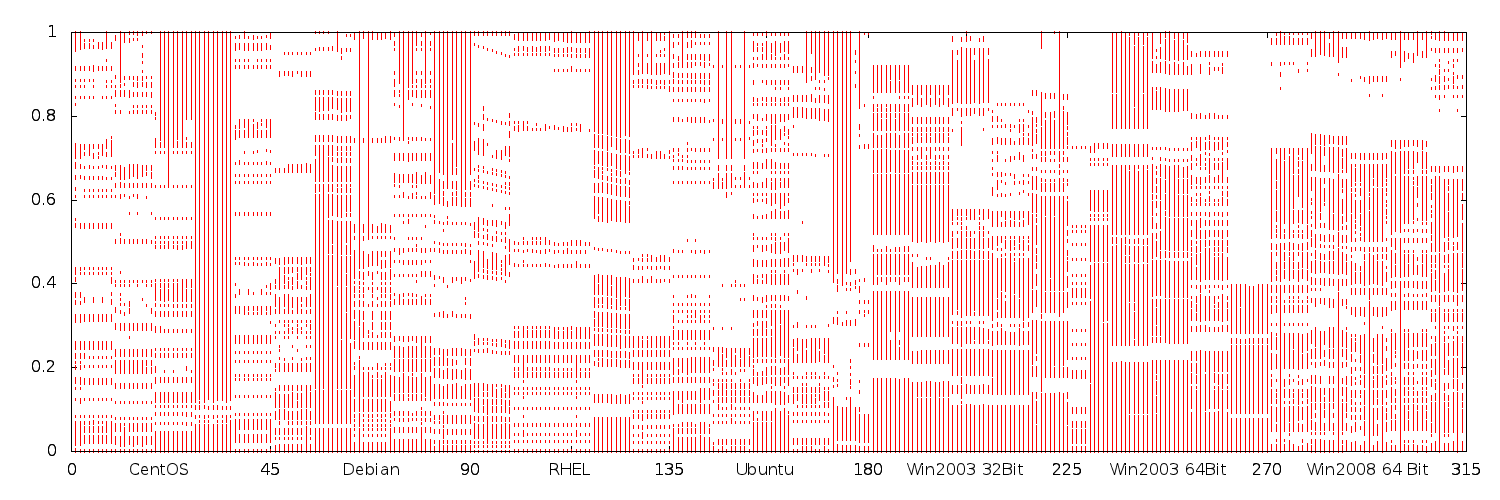
\includegraphics[width=6.5in,height=2in]{countmodify.png}
  %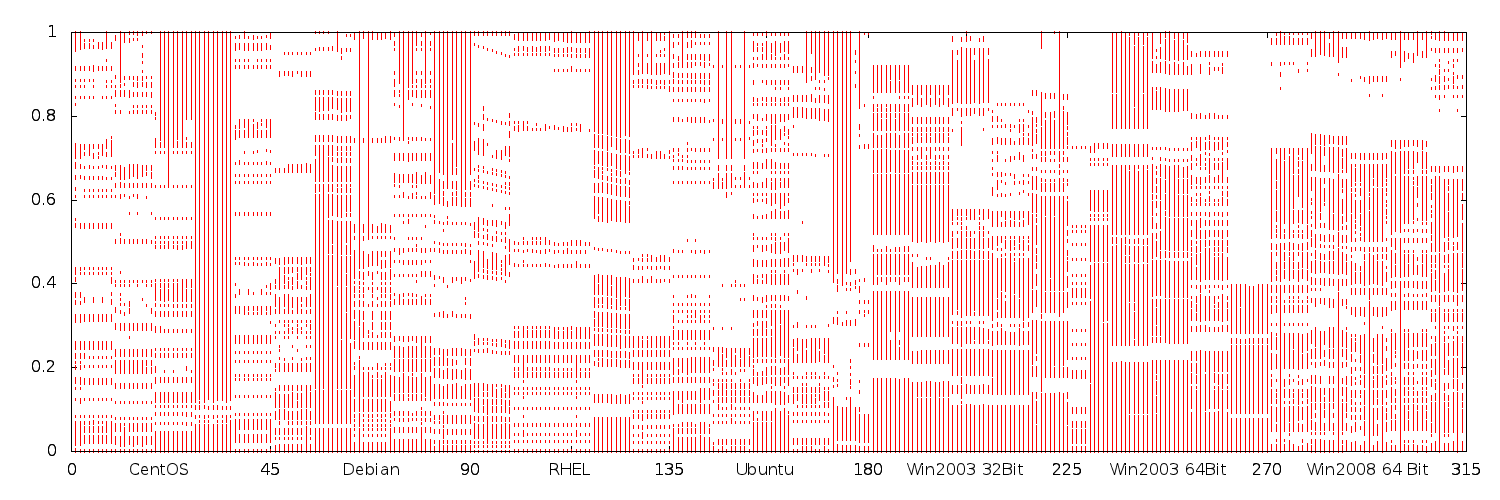
\epsfig{file=countmodify.eps, width=6.5in}
\caption{Bitmaps of dirty pages between snapshots}
\label{fig:dirty}
\end{figure*}

\begin{table}[htb]
  \centering
    \begin{tabular}{|l|p{1.3in}|p{0.4in}|}
        \hline
        OS Type & After Reduction Within \newline Dirty Page (GB) & Ratio \\ \hline
        Debian & 161.11 & 6.42 \\ \hline
        Ubuntu & 145.02 & 6.82 \\ \hline
        RHEL & 185.34 & 5.43 \\ \hline
        CentOS & 479.78 & 2.03 \\ \hline
        Win2003 32Bit & 80.14 & 7.87 \\ \hline
        Win2003 64Bit & 95.07 & 8.35 \\ \hline
        Win2008 64Bit & 172.22 & 9.76 \\ \hline
        Combined & 1318.68 & 5.26 \\
        \hline
    \end{tabular}
    \caption{Data reduction via 4KB block deduplication within dirty pages}
    \label{tab:locality}
\end{table}

\emph{Observarion 6: Data reduction ratio is generally improved, but there is still lots of
improvment space compare to complete deduplication.} We see significant improvment for all OS
types, which definitely deserves adding an additional layer to dirty-page based 
data reduction. In addition, the cost of looking one page's block hash index
shall be very small compare to full hash index lookup.

However, this is probably the best of what we can get from locality. The rest of
duplication mainly lies between VMs, e.g., same or slightly different versions of OS distributions, 
similar software installations, etc. Such duplications can not be easily 
eliminated and worth further research efforts.
 %
\section{Duplication V.S. Scale}
Dealing with large scale VM cloud, one of the most important questions is
whether data duplication will grow with the system scale. 
One hypothesis we have is that when the total number of block increases,
the chance that it being duplicated with another is going to be higher. Thus
we shall get better data reduction with larger scale of data.
Past study\cite{keren08} has suggested that virtual disks with 
operating systems installed should share large amount of software related data,
which indirectly supports this argument.
However, some other data study\cite{middleware11} showed the opposite.

In this experiment we test the complete deduplication under the scenario
that no snapshot backup is involved. To simulate the scale factor,
we start with partial data sets and scale them up by adding disk images.
Complete deduplication is performed at each stage to examine the reduction ratio.
Our DDS data set already contains no snapshot backup data. For VOSS, we simply pick
the earliest snapshot for each VM.

\begin{figure}
  \centering
  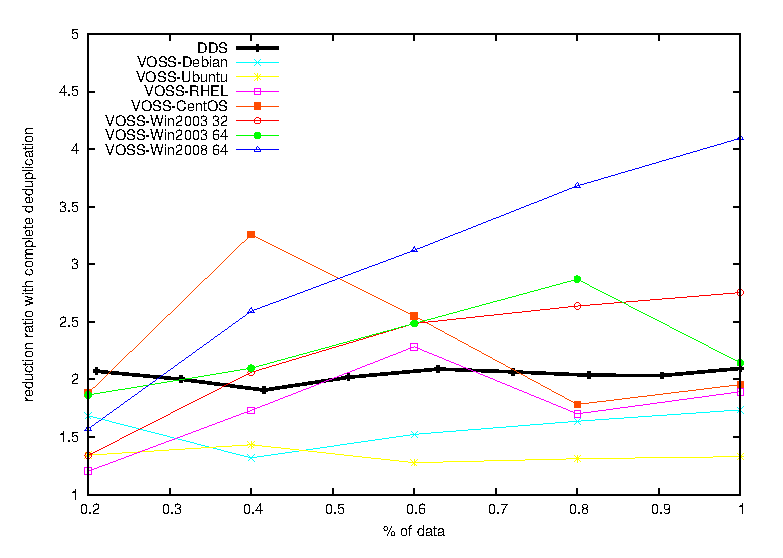
\epsfig{file=dedup_ratio.eps, width=3.2in}
  \caption{Reduction ratio of complete deduplication at different scale}
  \label{fig:scale}
\end{figure}

\emph{Observation 7: Reduction ratio by complete deduplication does not appear to increase with storage scale.}
In general we see almost no increment of reduction ratio along with the data scale, especially
for user generated data, shown as DDS in Figure\ref{fig:scale}, its reduction ratio is always
near 2:1. For OS disks, some Windows distributions appear to have incremental reduction, which is suspected to
because the size of Windows system is much bigger than Linux, thus it has much more redundant
data that widely exist in all VMs. We expect to perform larger scale study on OS disks in future
to obtain better conclusion on this topic.
%\input{count} %data study, zipf, model of cds size and dedup efficiency
%\section{Results}
In our snapshot deduplication architecture, CDS is the key to achieve greater deduplication than
incremental backup solutions. Our basic assumption of CDS us that VM disks, especially OS disks,
have huge amount of data in common, and such common data can be represented by a relatively smaller data set
because of their high appearence frequency. As a result, the major portion of snapshot deduplication effect shall 
emerge from eliminating the duplication of such a small data set. In this section, we evaluate
the effectiveness of CDS using real user VM disks from our production VM cluster.

\subsection{Experiment Setup}
The data set we use is the same as described in previous section. 
We choose extreme binning and perfect deduplication to compare against.
In all experiments, our deduplication enforces 2MB fix-sized segment boundary, 
and uses TTTD algorithm to divide segment into 4KB variable-sized blocks.
For perfect deduplication and extreme binning, the whole snapshots are splitted
using TTTD with 4KB average size. The original extreme binning paper uses whole file
as the input unit, but that is way too big for our system. 
Thus we split image snapshot files into variable-sized segments base on the block hash list, 
using TTTD with average size of 2MB.

\subsection{OS Disk}
We extract the CDS of OS disks by counting the blocks that will appear in a VM's
block store if no CDS is involved in the deduplication process. The threshold is set to less than
1.5\%, which is quite sufficient to include the OS related data since their duplication is much
heavier than others. Then we use this CDS to run the deduplication process again.
Finally we extracted about 80GB of CDS data from 350 OS disk snapshots,
the corresponding CDS meta occupies 800MB in CDS cache.

\begin{figure}
  \centering
  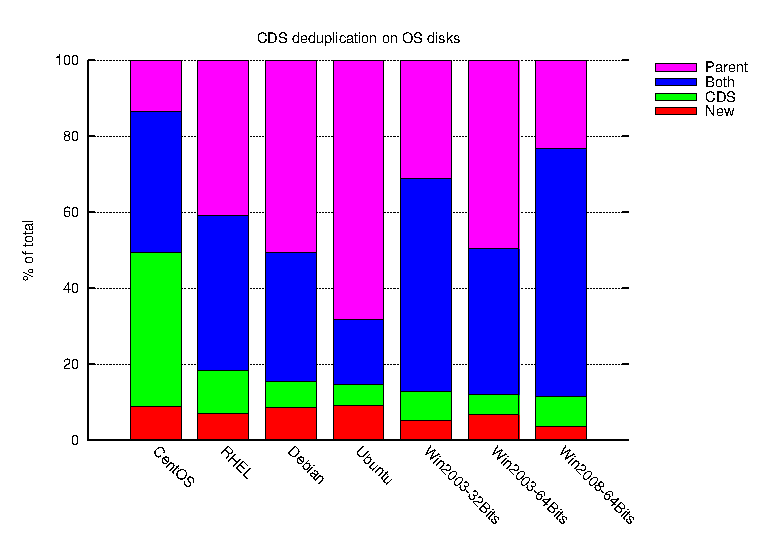
\epsfig{file=images/os_cds_sim.eps, height=2in, width=2.66in}
  \caption{CDS deduplication effect on OS disks}
  \label{fig:oscds}
\end{figure}

For each block, we tag it with one of the following:
\begin{itemize}
\item {New: this block cannot be deduplicated and thus write to block store.}
\item {CDS: this block is deduplicated by CDS.}
\item {Parent: this block is not found in CDS, but is found in parent snapshot's segment recipe.}
\item {Both: this block is both found in CDS and parent snapshot.}
\end{itemize}
As we can see from \ref{fig:oscds}, locality dominates.
This is because the interval between two snapshots is quite short due to our daily snapshot strategy. 
However, locality still doesn't work well on some of the OSes. But CDS, on the contrary,
finds a lot of duplicates that locality can't find, especially in a VM's first snapshot.

Combining all the VMs, we see the overall 7.4TB of data is reduced to 512GB. Extreme bining 
reduces this data set to 542GB, which is slightly worse. As a reference, perfect deduplication achieves
364GB in this experiment.

Overall, none of locality or CDS can solely work well, but by combining them together 
we get fairly good and stable deduplication ratio to all kind of OSes. If compare to all
incremental backup solutions, CDS can save addition 50\%+ of disk space because it greatly reduces
the cross-VM duplicates.

\subsection{Data Disk}
Figure \ref{fig:pd} shows the compression ratio of perfect deduplication at different data scales. 
Basically perfect deduplication would help us save 50\% of space on user data, 
regardless of scale. If we put all these unique data into CDS, we could achieve perfect deduplication, 
which is not affordable. So we need to see how much space saving of perfect 
deduplication can be achieved through a limit size CDS.
\begin{figure}
  \centering
  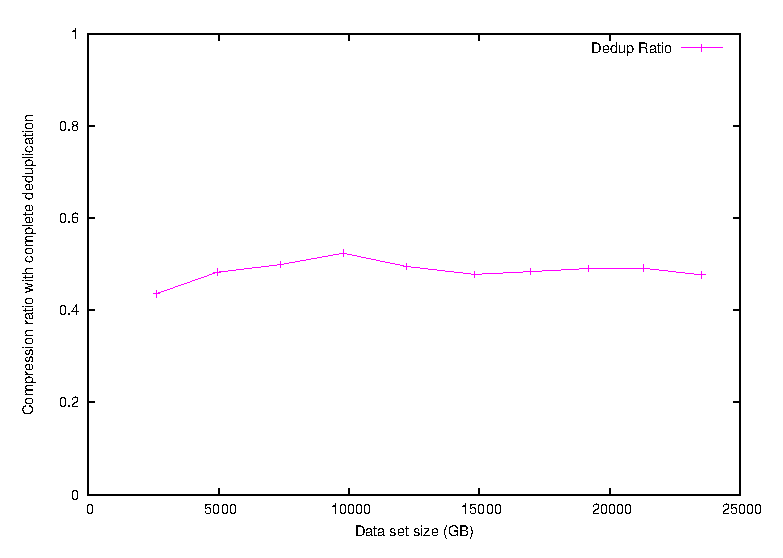
\epsfig{file=images/dedup_ratio.eps, height=2in, width=2.66in}
  \caption{Perfect deduplication on data disks}
  \label{fig:pd}
\end{figure}

We rank unique data blocks by their duplication count, 
and choose the hottest blocks as CDS. 
We define \emph{space saving ratio} as the space saving of CDS divide by 
perfect deduplication saving. Figure \ref{fig:datacdssize} shows the relationship between CDS size and space saving. 
It’s clear a very small amount of CDS data provides more than 50\% saving. 
But this effect decreases when more data are added to CDS. 
The lower bound of CDS space saving ratio is 50\%, which is very easy to accomplish. 

\begin{figure}
  \centering
  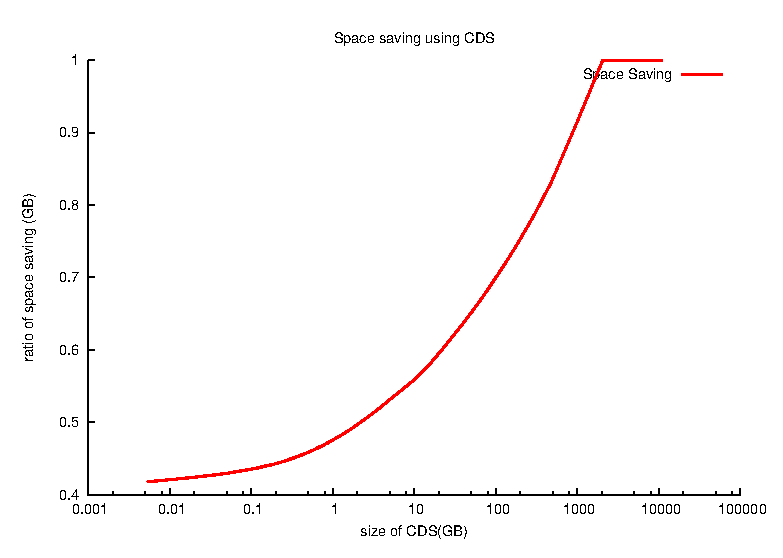
\epsfig{file=images/uniquedata-saving.eps, height=2in, width=2.66in}
  \caption{Size of CDS vesus space saving}
  \label{fig:datacdssize}
\end{figure}

The upper bound of CDS size is restricted by system memory resource.
Figure \ref{fig:datacds} shows how CDS space saving is affected by the system scale. 
In this experiment we first set out a goal of space saving ratio, 
then we watch how much data we need to put into CDS to achieve this goal.
From the graph we can see a 75\% saving goal lead to a stable ratio between 
CDS size and data size, which requires 0.01\% of data to be put in CDS.

Base on above data we can estimate the size of data CDS and its effect. 
Currently we prepared 500MB memory per machine to store CDS meta, then it can represent 50GB of data. 
If we assume each VM has 30GB of user data at runtime, and we host 25 VMs per machine, 
 maintain 10 snapshots per VM, each brings 10\% additional modified data. 
Thus the user data in snapshot system is 1.5TB per machine. So the upper bound of 
$CDS size/ Data size = 0.033$, which is sufficient for the 75\% saving goal.

\begin{figure}
  \centering
  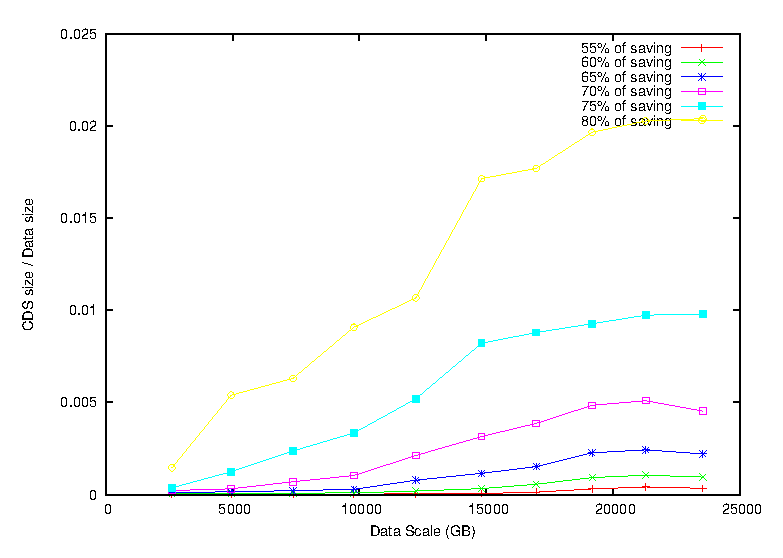
\epsfig{file=images/cds_scale.0.7.eps, height=2in, width=2.66in}
  \caption{CDS deduplication effect on data disks}
  \label{fig:datacds}
\end{figure}

Unlike the CDS of OS disks which is mainly composed of OS related data thus highly predictable, 
data disks is unpredictable because we cannot control what user can put in there. But we still
suspect that highly duplicated data in existing data are very likely to be duplicated again.
So we randomly pick 50 out of 1322 data disks as the new data, and use the rest as existing data
to extract CDS. Using 1.5\% as CDS threshold, we see the total 1198GB of new data is reduced by 
755.8GB, while perfect deduplication can reduce 1017.4GB. So 74.3\% of duplicate blocks are eliminated 
by pre-trained CDS, which is quite satisfiable.

%\section{Related Works}
Several approaches have been previously proposed to enable efficient deduplication in D2D backup.

DDFS\cite{bottleneck08} exploits chunk locality to achieve high-throughput perfect deduplication. 
It preserves locality by a Stream-Informed Segment Layout and exploits locality with Locality Preserved Cache. 
An in-memory Bloom Filter is also used to accelerate non-duplicate chunk identification.

Sparse Indexing\cite{sparseindex09} is an approximate deduplication technique designed for D2D backup. 
It divides data stream into variable-sized multiple kilobytes chunks, and construct multiple megabytes segments
using the same chunking technique, 
which are then sampled and mapped to a compact in-memory sparse index. 
Incoming segments are only deduplicated against several existing similar 
segments selected according to the sparse index.

Both DDFS and Sparse Indexing are designed for D2D backup workloads, 
and do not address the scalability issue in a distributed environment. 
A few scalable deduplication approaches have been proposed recently.

Extreme Binning\cite{extreme_binning09} is a scalable parallel deduplication approach 
that targets at non-traditional backup workloads that consist of low-locality individual files. 
It groups highly similar files into bins, and eliminates duplicate chunks inside each bin. 
Duplicate chunks are allowed to exist among different bins, resulting in approximate deduplication. 
By keeping only the primary index in memory, Extreme Binning can reduce the RAM requirement while 
maintaining a reasonably high throughput. However, their per-file based similarity detection 
is going to group all similar files into one node, which will break load balancing if some files are
huge and similar(e.g., virtual machine images).

MAD2\cite{mad210} is a scalable high-throughput exact duplication approach. 
MAD2 utilizes on-disk Hash Bucket Matrix to preserve fingerprint locality and 
integrates in-memory Dual Cache to capture and exploit locality. 
In addition, MAD2 employs Bloom Filter Array to efficiently identify unique 
incoming fingerprints and indicate where a duplicate may reside. 
By employing a DHT-based Load-Balance technique to distribute file recipes 
and chunk contents among multiple storage nodes in their backup sequences, 
MAD2 further enhances performance with a well balanced load. However, the
data locality does not exist for cloud storage because only changed chunks are expected
to be uploaded, and
the heavy usage of memory and CPU indicates such exact deduplication backup systems
need storage-exclusive servers with hardware replication support, which is not a general case 
for the cloud..

HYDRAstor\cite{hydrastor09}, a scalable secondary storage solution, 
constructs its backend using a grid of storage nodes built around a distributed hash table. 
The backend maintains large-scale variable-sized, content-addressed, immutable, 
and highly-resilient data blocks that are logically organized in a directed acyclic graph. 
Duplicate chunks are eliminated according to their hashes. 
HYDRAstor adopts an average chunk size of 64KB, among other constraints, 
to keep all the metadata in memory and avoid the duplicate-lookup disk bottleneck. 
This degrades the space efficiency of deduplication, and still requires huge amount of memory.

We believe a deduplication backend of cloud storage must have scalability and
 high availability built in mind, being able to run on low-cost non-proprietary machines.
  Unlike sloud, all above systems lack one or a few such properties. All exact deduplication approaches
are too costly, this is why we choose similarity based approach to trade deduplication
accuracy for speed. 

Eariler deduplication systems mainly focus on improving storage space efficiency by eliminating 
duplicates at the file level, fixed-size block level, or variable-sized chunk level. 
EMC's Centera\cite{emc_centera} identify and eliminate duplicate data by comparing 
the hash of the whole file or fixed content. Venti\cite{venti02}, a block-level archival storage, 
removes redundant fixed-size data blocks by comparing their secure hashes. Pastiche\cite{pastiche02} 
utilizes chunk-level duplicate detection to construct a resource-saving peer-to-peer backup network. 
Deep Store\cite{deepstore05}, a large scale archival storage system, uses both variable-sized 
chunk-level deduplication and delta compression to save storage. Jumbo Store\cite{jumbo07} organizes 
variable-sized chunks into Hash-Based Directed Acyclic Graphs to save both storage and 
bandwidth while performing incremental upload and versioning for a utility rendering service. 

Duplicate detection technique has also been used in bandwidth-saving synchronization protocols\cite{rsync} 
and low-bandwidth network file systems\cite{lbfs01}.
%\section{Conclusion}
In this paper we present a new parallel deduplication technique for VM cloud.
Our technique utilizes the special data characteristic in VM cloud backup system
to accommodate very limited resources for data deduplication.
By storing the commonly used OS related data, and the hottest user generated data, 
we greatly reduce the cross-VM data duplication in VM snapshot backups. Experiments show
our solution can eliminate the majority of data duplication with a tiny fraction of
block hash index store in memory. It does not only saves valuable system resouces in
the VM cloud, but also makes deduplication much faster.

%\section{Conclusion}
\label{sect:final}
In this paper we propose a VM-centric deduplication scheme for 
VM snapshot backup in the cloud for maximizing fault isolation and tolerance. 
Inner-VM deduplication localizes backup data dependency and exposes more parallelism  
while cross-VM deduplication with a small common data set
effectively  covers a large percent of duplicate data.
The scheme organizes the write of small data chunks into large file system blocks so
that each underlying file block is associated with one VM for most cases.
by keeping most of the FSBs only referenced by 1 VM, we isolate faults and improve overal fault tolerance.
Our solution accomplishes reasonable and competitive deduplication efficiency while
still meeting stringent cloud resource usage requirements. 
Our analysis shows that  this VM centric scheme 
can  provide  better fault tolerance than VM-oblivious global deduplication schemes
while using a small amount of computing and storage resources. 


[Talk about more what we learn from Evaluation]
Evaluation using real user's VM data shows
our solution can accomplish 92\% of what complete global
deduplication can do. 
Compare to today's widely-used snapshot technique, our scheme reduces almost
two-third of snapshot storage cost.
Finally, our scheme uses a very small amount of memory on each node, and leaves
room for additional optimization we are further studying.


%This paper studies a cluster-based VM-centric scheme which collocates a lightweight
%backup service with the cloud service and it integrates multiple duplicate detection strategies that  
%localize the deduplication as much as possible within each virtual machine.
%This  paper  provides a comparative evaluation of this scheme in  accomplishing a high deduplication 
%efficiency while sustaining a good backup throughput. 

%This paper studies the      a VM snapshot storage architecture which adopts multiple-level selective deduplication to bring the benefits of fine-grained data reduction into cloud backup storage systems.
%In this work, we describe our working snapshot system implementation, and provide
%early performance measurements for both deduplication impact and
%snapshot operations.

\comments{
\section*{Acknowledgments}
{
We would like to thank Weicai Chen and Shikun Tian from Alibaba for their kind support, 
and the anonymous referees for their comments.
Wei Zhang has received internship support from Alibaba  for VM backup system development.
This work was supported in part by NSF IIS-1118106.
Any opinions, findings, and conclusions or recommendations expressed in this material are those of the authors and
do not necessarily reflect the views of Alibaba or the National Science Foundation.
}
}
%Noted that 6\% is still significant, which is about 24GB per each VM and for a 1000 node Aliyun cluster,
%this is about 600 terabytes.
 
%Our experiments show th
%our solution can eliminate the majority of data duplication with a tiny fraction of
%block hash index store in memory. It does not only saves valuable system resouces in
%the VM cloud, but also makes deduplication much faster.
%
%
%Using  50 user VM data out of 1322 data disks as the training data and
%with  1.5\% as PDS threshold, we see the total 1198GB of new data is reduced by
%755.8GB, while perfect deduplication can reduce 1017.4GB. So 74.3\% of duplicate blocks are eliminated
%by pre-trained PDS, which is quite satisfactory.



      %\setlength{\itemsep}{ex}%
%      \setlength{\parskip}{0ex}%
%\setlength{\itemsep}{-3mm}

	%\linespread{0.3} 
%  \let\oldthebibliography=\thebibliography
%  \let\endoldthebibliography=\endthebibliography
%  \renewenvironment{thebibliography}[1]{%
%    \begin{oldthebibliography}{#1}%
%      \setlength{\parskip}{-0.02ex}%
%      \setlength{\itemsep}{-0.02ex}%
%      \setlength{\baselineskip}{-0.02ex}%

%  }%
%  {%
%    \end{oldthebibliography}%
%  }
{\small
\bibliographystyle{abbrv}
\bibliography{dedup,dedup1}
}
\end{document}
